\subsection{Address Translation Attacks}
\label{sec:paging_attacks}

\S~\ref{sec:system_software_attacks} argues that today's system software is
virtually guaranteed to have security vulnerabilities. This suggests that a
cautious secure architecture shoild avoid having the system software in the
TCB.

Removing the system software from the TCB means that the architecture must
provide a method for running application code inside a container that is
isolated from the untrusted system software. One of the more difficult problems
these designs must solve is that application software relies on the memory
management services provided by the system software, which is now untrusted.

Intel's SGX~\cite{mckeen2013sgx, anati2013sgx}, which was inspired by
Bastion~\cite{champagne2010bastion}, leaves the system software in charge of
setting up the page tables (\S~\ref{sec:paging}) used by address translation,
but instates access checks that prevent the system software from directly
accessing the isolated container's memory.

This section discusses some attacks that become relevant when the application
software does not trust the system software which in charge of the page tables.
Understanding these attacks is a prerequisite to reasoning about the security
properties of architectures with this threat model. For example, a large amount
of the mechanisms in SGX are aimed at dealing with a subset of the attacks
described here.


\subsubsection{Passive Attacks}
\label{sec:fault_tracking_attacks}

System software uses the the CPU's address translation feature
(\S~\ref{sec:paging}) to implement page swapping, where infrequently used
memory pages are evicted from DRAM to a slower storage medium. Page swapping
relies the accessed (A) and dirty (D) page table entry attributes
(\S~\ref{sec:page_table_attributes}) to identify the DRAM pages to be evicted,
and on a page fault handler (\S~\ref{sec:faults}) to bring evicted pages back
into DRAM when they are accessed.

Unfortunately, the features that support efficient page swapping turn into a
security liability, when the system software managing the page tables is not
trusted by the application software using the page tables. The system software
can be prevented from reading the application's memory directly by placing the
application in an isolated container. However, the untrusted system software
can still infer partial information about the application's memory access
patterns, by observing the application's page faults and page table attributes.

We consider this class of attacks to be passive attacks that exploit the CPU's
address translation feature. It may seem that the page-level memory access
patterns provided by these attacks are not very useful. However,
\cite{xu2015pagefaults} describes how this attack can be carried out against
Intel's SGX, and implements the attack in a few practical settings. In one
scenario, which is particularly concerning for medical image processing,
the outline of a JPEG image is inferred while the image is decompressed inside
a container protected by SGX's isolation guarantees.


\subsubsection{Active Attacks}
\label{sec:memory_mapping_attacks}

Figure~\ref{fig:sgx_mapping_attack} shows a hypothetical memory mapping attack.
Understanding this type of attack
greatly increases one's ability to reason about SGX's security.

\begin{figure}[hbt]
  \centering
  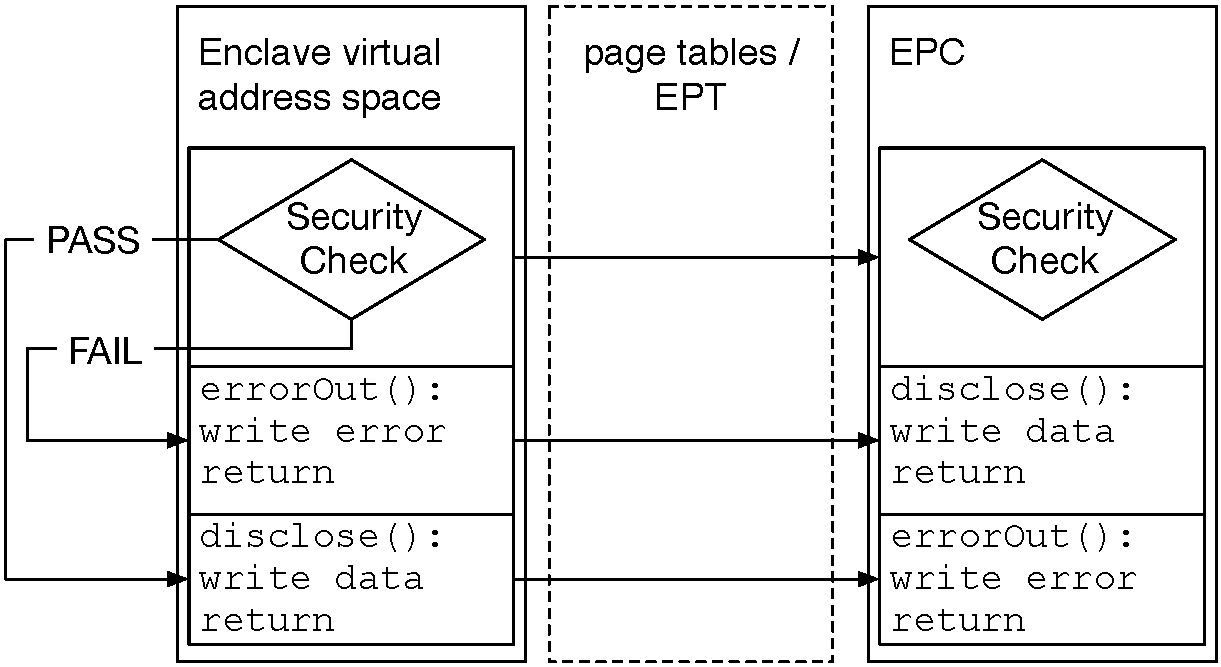
\includegraphics[width=85mm]{figures/sgx_mapping_attack.pdf}
  \caption{
    An example of a memory mapping attack, which is prevented by SGX. The
    enclave's author intends to disclose a piece of sensitive information only
    when a security check passes. Malicious system software maps the virtual
    address of the procedure called when the security check fails to an EPC
    page that contains the procedure that discloses the sensitive information,
    which is supposed to be called when the security check passes.
  }
  \label{fig:sgx_mapping_attack}
\end{figure}

For simplicity, we assume an enclave that performs a security check to decide
whether to disclose some sensitive information. Depending on the security
check's outcome, the enclave code either calls a \texttt{errorOut} procedure,
or a \texttt{disclose} procedure. We furthermore assume that each procedure's
code starts at a 4KB boundary, and takes up less than 4KB, so each procedure
fits in an EPC page. These requirements seem unrealistic, but the underlying
attack remains an issue in real applications.

In a memory mapping attack, malicious system software sets up the page tables
or EPT in such a way that the virtual address intended to store the
\texttt{errorOut} procedure is actually mapped to an EPC page that contains the
\texttt{disclose} procedure. Without any security measures in place, the
enclave would execute the \texttt{disclose} code and reveal sensitive
information, even though the security check fails.

The SGX security mechanisms, explained throughout the rest of this paper,
prevent enclave code execution if a memory mapping attack occurs. Therefore,
SGX prevents malicious system software from directly obtaining sensitive
information via memory mapping attacks.
